\begin{figure*}[t]
%\vspace{-.1cm}
\centering
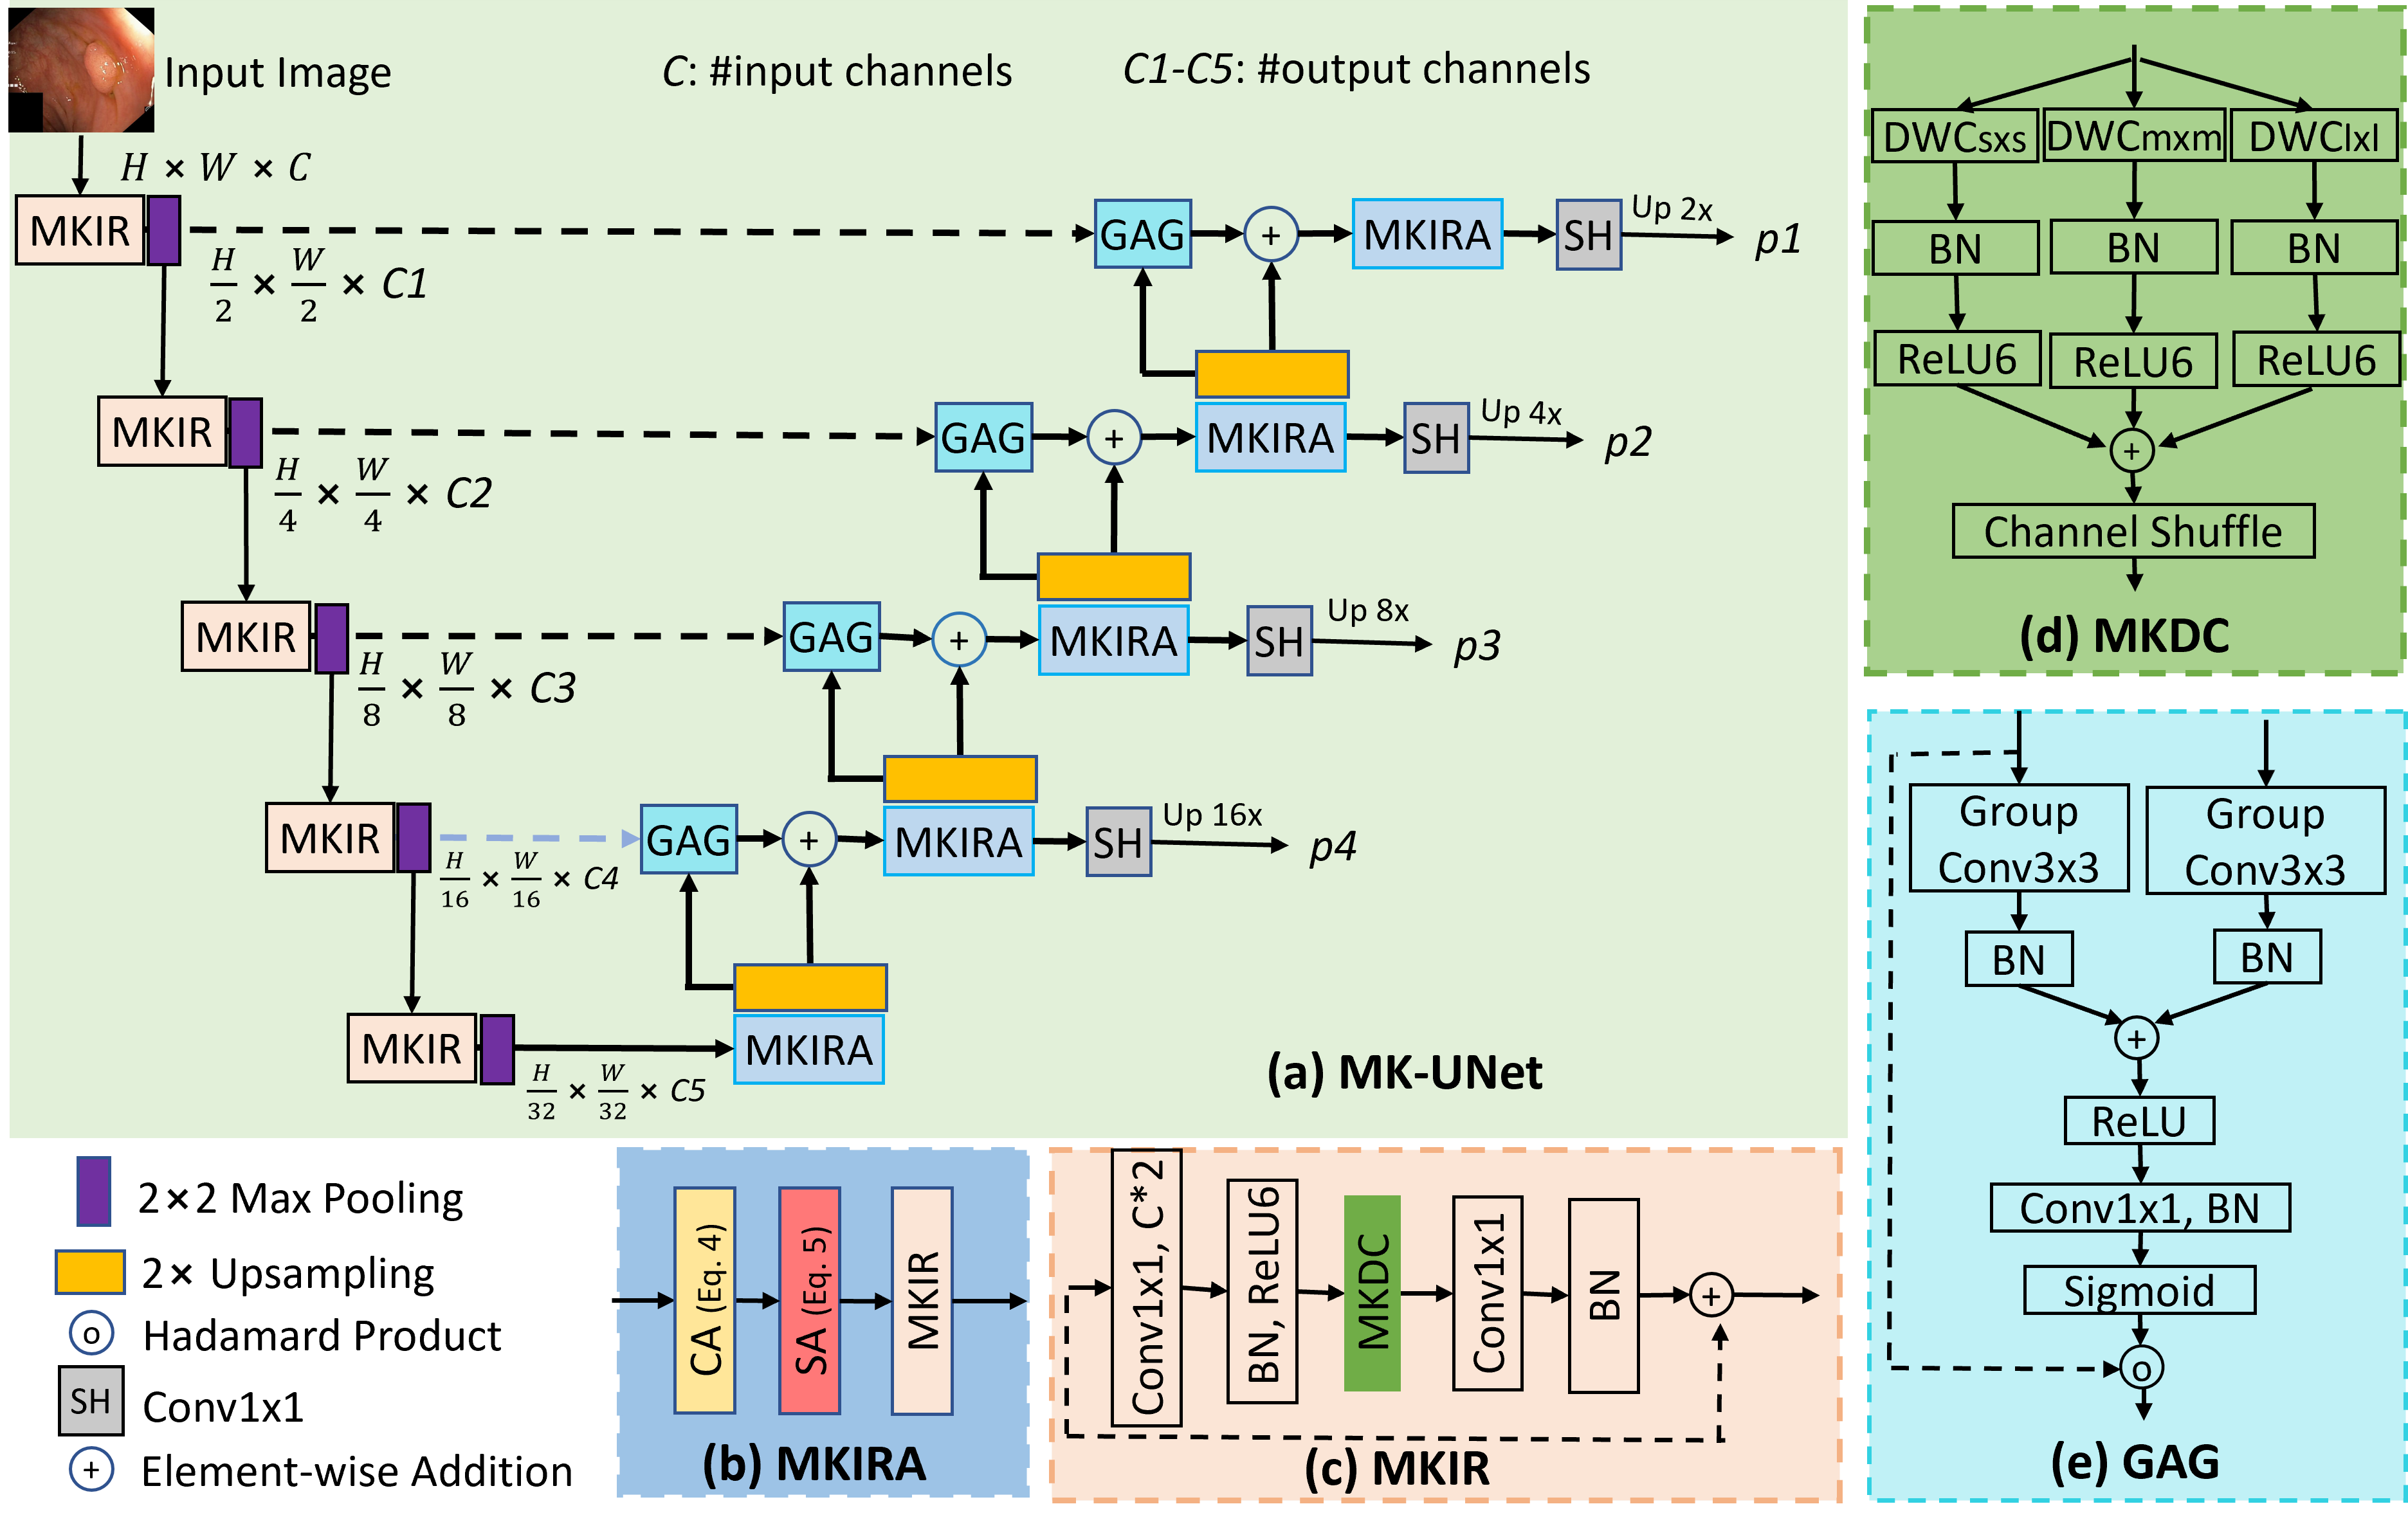
\includegraphics[width=0.88\textwidth]{sections/imgs/mk_unet_architecture.png}
\vspace{-.2cm}
\caption{The proposed network diagram. (a) Five-stage MK-UNet network (b) Multi-kernel inverted residual attention (MKIRA), (c) Multi-kernel inverted residual (MKIR), (d) Multi-kernel (parallel) depth-wise convolution (MKDC), (e) Grouped attention gate (GAG). p1, p2, p3, and p4 are output segmentation maps. \textbf{Note}: Channel attention (CA), Spatial attention (SA).}
\label{fig:architecture}
\vspace{-.2cm}
\end{figure*}

\section{Method}
\label{sec:method}
We describe next our core building blocks. Then, we introduce our MK-UNet architecture by integrating these blocks into the baseline UNeXt \cite{valanarasu2022unext} (Fig. \ref{fig:architecture}a in green box). %Different components are described below.

\subsection{Multi-kernel Inverted Residual (MKIR)} 
We first introduce the multi-kernel inverted residual ($MKIR$) block to generate and refine feature maps (Fig. \ref{fig:architecture}c). By utilizing multiple (same or different) kernel sizes, $MKIR$ allows for better understanding of both fine-grained details and broader contexts, thereby enabling a comprehensive representation of the input. As shown in Fig. \ref{fig:architecture}c, the process begins by expanding the \#channels (i.e., expansion\_factor = 2) through point-wise convolution $PWC_1$, batch normalization $BN$ \cite{ioffe2015batch}, and $ReLU6$ activation \cite{krizhevsky2010convolutional}. This is followed by multi-kernel depth-wise convolution $MKDC$ for capturing application-specific complex spatial contexts. A subsequent point-wise convolution $PWC_2$ and $BN$ restore the original \#channels. The MKIR (Eq. \ref{eq:mkir}) significantly reduces the computational cost while ensuring rich feature representation: %\scriptsize
\begin{equation}
%\vspace{-.05cm}
\scalebox{0.75}{\(
    MKIR(x) = BN(PWC_2(MKDC(ReLU6(BN(PWC_1(x))))))
\)}
%\vspace{-.05cm}
    \label{eq:mkir}
\end{equation}
%\normalsize
where $MKDC$ for multiple kernels ($K$) is defined in Eq. \ref{eq:mkdc} and Fig. \ref{fig:architecture}d: %\vspace{-.05cm}
\begin{equation}
    \scalebox{0.9}{\( 
    MKDC(x) = CS(\sum_{k \in K} DWCB_{k}(x))
    \)}
    %\vspace{-.05cm}
    \label{eq:mkdc}
\end{equation}
where $DWCB_{k}(x) = ReLU6(BN(DWC_{k}(x)))$. Here, $DWC_{k}$(.) is a depth-wise convolution with the kernel $k\times k$. To address the channel independence in depth-wise convolution, a channel shuffle ($CS$) is used to ensure the inter-channel information flow. Our $MKDC(.)$ differs from $MSCB$ (in EMCAD \cite{rahman2024emcad}) in their core theoretical concepts. Our multi-kernel trick supports both $k_1=k_2$ (same-size kernels) and $k_1 \neq k_2$ (different-size kernels) for $k_1, k_2 \in K$ versus conventional multi-scale (only $k_1 \neq k_2$) designs \cite{rahman2024emcad, lin2023scale, seo2022spatial}, thus allowing adaptable context extraction.
This conceptual distinction allows MK-UNet to adapt kernel sizes based on application-specific needs (e.g., large kernels for large objects, small kernels for small objects, or mixed for both objects segmentation).  %Additionally, our sequential $MKDC$(.) uses the recursively updated input $x$, where the input $x$ is residually connected to the previous $DWCB_{ks}$(.) for better regularization as in Eq. \ref{eq:msdc_sequential}: 
%\vspace{-.2cm}
%\begin{equation}
%    x = x + DWCB_{ks}(x)
%    \vspace{-.2cm}
%    \label{eq:msdc_sequential}
%\end{equation}
%\vspace{-.4cm}

%\vspace{-.4cm}
\subsection{Multi-kernel Inverted Residual Attention (MKIRA)}
We present a lightweight multi-kernel inverted residual attention, MKIRA, to refine the feature maps ($x$). MKIRA uses channel attention ($CA$) \cite{hu2018squeeze} to focus on relevant channels, a spatial attention ($SA$) \cite{chen2017sca} to capture the local context, and a multi-kernel inverted residual ($MKIR$) to enrich the feature maps while capturing contextual relationships. The $MKIRA$ (Fig. \ref{fig:architecture}b) is given in Eq. \ref{eq:mkira}: 
%\vspace{-.25cm}
\begin{equation}
    MKIRA(x) = MKIR(SA(CA(x)))
    %\vspace{-.2cm}
    \label{eq:mkira}
\end{equation}
%where $x$ is the input tensor. Employing depth-wise convolution with multiple kernels, MKIRA achieves significant computational efficiency.

%\vspace{-.4cm}

%\vspace{-.8cm}
\noindent \textit{Channel Attention (CA):} 
%We use channel attention block to assign different levels of importance to each channel, thus emphasizing more relevant features while suppressing less useful ones. Basically, the CA identifies \textit{which feature maps} to focus on (and then refine them). Following \cite{woo2018cbam}, in CA, we first apply the adaptive maximum pooling ($P_m$(·)) and adaptive average pooling ($P_a$(·)) to the spatial dimensions (i.e., height and width) to extract the most significant feature of the entire feature map per channel. Then, for each pooled feature map, we reduce the number of channels $r=16$ times separately using a point-wise convolution ($C_1$(·)) followed by a ReLU activation ($R$). Afterward, we recover the original channels using another point-wise convolution ($C_2$(·)). We then add both recovered feature maps and apply Sigmoid ($\sigma$) activation to estimate attention weights. Finally, we incorporate these weights to input $x$ using the Hadamard product ($\circledast$). The $CA$(·) (Fig. \ref{fig:architecture}(f)) is defined using Eq. \ref{eq:ca}: 
We use $CA$ \cite{hu2018squeeze} to enhance relevant features by applying adaptive max ($AMP$) and average pooling ($AAP$) to condense the spatial information \cite{Rahman_2023_WACV}; this is followed by channel reduction ($r = 16$) through point-wise convolution $PWC_1$ with $ReLU$ ($R$) activation \cite{nair2010rectified} and expansion through $PWC_2$. The $Sigmoid$ ($\sigma$) activation generates attention weights, which are then applied to the input via the Hadamard product ($\circledast$), while focusing on crucial feature maps. The $CA$ is defined in Eq. \ref{eq:ca}:%\vspace{-.2cm}
 %\small 
 \begin{equation}
 \scalebox{0.62}{\( CA(x)=\sigma(PWC_2(R(PWC_1(AMP(x))))+PWC_2(R(PWC_1(AAP(x))))) \circledast x
 \)}
 %\vspace{-.25cm}
    \label{eq:ca}
\end{equation}
%\normalsize
%where $\circledast$ is the Hadamard product. 
%$\sigma$(·) is the Sigmoid activation. $P_m$(·) and $P_a$(·) denote adaptive maximum pooling and adaptive average pooling, respectively. $C_1$(·) is a convolutional layer with $1 \times 1$ kernel size to reduce the channel dimension 16 times. $R$ is a ReLU activation layer and $C_2$(·) is another convolutional layer to recover the original channel dimension. 
%\vspace{-.8cm}

\noindent \textit{Spatial Attention (SA):} 
%We use spatial attention to mimic the attentional processes of the human brain by focusing on specific parts of an input image. Basically, the SA determines \textit{where} to focus in a feature map; then it enhances those features. This process enhances the model's ability to recognize and respond to relevant spatial features, which is crucial for image segmentation where the context and location of objects significantly influence the output. In SA, we first pool maximum ($Channel_{max}$(·)) and average ($Channel_{avg}$(·)) values along the channel dimension to pay attention to local features. Then, we use a large kernel (i.e., $7 \times 7$ as in \cite{dong2021polyp}) convolution layer $LKC$(.) to enhance local contextual relationships among features. Afterward, we apply the Sigmoid activation to calculate attention weights. Finally, we feed these weights to the input $x$ (using Hadamard product ($\circledast$) to attend information in a more targeted way. The $SA$(.) (Fig. \ref{fig:architecture}(g)) is defined using Eq. \ref{eq:sa}:
We use $SA$ \cite{chen2017sca} to focus on specific image regions to highlight key features, crucial for accurate segmentation. The $SA$ aggregates maximum ($Ch_{max}$) and average ($Ch_{avg}$) channel values to highlight local details, then it employs a large-kernel ($7 \times 7$) convolution ($LKC$) to strengthen the contextual connections. The $Sigmoid$ ($\sigma$) activation derives attention weights, applied to the input $x$ via the Hadamard product ($\circledast$), ensuring targeted refinement. The $SA$ is derived in Eq. \ref{eq:sa}:
%\vspace{-.2cm}
\begin{equation}
    SA(x) = \sigma(LKC([Ch_{max}(x), Ch_{avg}(x)])) \circledast x
    %\vspace{-0.2cm}
    \label{eq:sa}
\end{equation}
\normalsize

%\vspace{-.5cm}
\subsection{Grouped attention gate (GAG)}
We use a grouped attention gate ($GAG$, Fig. \ref{fig:architecture}e) that mixes the feature maps with the attention coefficients for enhancing the relevant features and suppressing the irrelevant ones. By utilizing a gating signal from higher-resolution features, $GAG$ directs the information flow, thus improving medical image segmentation accuracy. Unlike Attention UNet \cite{oktay2018attention}, which processes signals with $1\times1$ convolution, our method applies $3\times3$ group convolutions ($GC$) to both gating ($g$) and input ($x$) feature maps separately \cite{rahman2024emcad}. After convolution, the features undergo batch normalization ($BN$) and get combined via addition, followed by $ReLU$ ($R$) activation. Subsequently, a $1\times1$ convolution and batch normalization ($BN$) produce a unified feature map which, after the $Sigmoid$ activation ($\sigma$), generates the attention coefficients. These coefficients adjust the input feature $x$, and create an attention-enhanced output. $GAG$ is defined in Eq.s \ref{eq:ags_1}:% and \ref{eq:ags_2}:
%\vspace{-.1cm}
\begin{equation}
\scalebox{0.7}{\(
   GAG(g, x) = x \circledast \sigma(BN(Conv(R(BN(GC_g(g) + BN(GC_x(x)))))))))%q_{gag}(g, x))))
   \)}
   %\vspace{-.3cm}
    \label{eq:ags_1}
\end{equation} 
%\begin{equation}
%\scalebox{0.9}{\(
%    q_{gag}(g, x) = ReLU(BatchNorm(GroupConv_g(g) + BatchNorm(GroupConv_x(x)))))
%    \)}
%    %\vspace{-.25cm}
%    \label{eq:ags_2}
%\end{equation}
%\vspace{-.3cm}
%The $3\times3$ group convolutions in our GAG enhance the spatial context with lower computational cost, thus setting a new standard for gated feature map combination.

%Our implementation of $3\times3$ kernel group convolutions within $q_{gag}$(.) allows the GAG to access broader spatial contexts while minimizing computational demands, setting a new standard for feature map combination and attention gating in neural networks, particularly for enhancing medical imaging performance.

%\vspace{-.4cm}

%\subsection{Segmentation head (SH)}
%We use segmentation heads to produce the segmentation outputs from the refined feature maps of four stages of the decoder. The SH layer applies a $1\times1$ convolution $Conv_{1\times1}$(·) to the refined feature maps having $ch_i$ channels ($ch_i$ is the \#channels in the feature map of stage $i$) and produces output with \#channels equal to \#classes in target dataset for multi-class but $1$ channel for binary segmentation. The $SH$(·) is formulated as in Eq. \ref{eq:seg_head}:
%\begin{equation}
%    SH(x) = Conv_{1\times1}(x)
%    %\vspace{-0.1cm}
%    \label{eq:seg_head}
%\end{equation}

%\vspace{-.5cm}
\subsection{Multi-kernel UNet (MK-UNet)}
%Existing transformer-based models have limited (local) contextual information processing ability among pixels. As a result, the transformer-based model faces difficulties in locating the more discriminating local features. To address this issue, some works \cite{dong2021polyp,Rahman_2023_WACV, rahman2023multi} utilize computationally expensive 2D convolution blocks in the decoder. Although the convolution block helps to incorporate the local information, it results in long-range attention deficits. To overcome this problem, we propose a new cascaded graph convolutional decoder, G-CASCADE, for pyramid encoders.
%In this part, we introduce our multi-kernel UNet to process an image through multiple stages and produce high-resolution segmentation maps. As shown in Fig. \ref{fig:architecture}(a), MK-UNet has five encoder stages and five decoder stages. In each encoder stage, a multi-kernel inverted residual (MKIR) block is used to produce $C_i$ feature maps. Afterward, a Max Pooling layer is used to downsample the input by preserving important information. The feature map generated by the fifth stage of the encoder is fed into a multi-kernel inverted residual attention (MKIRA) block at the first stage of the decoder to robustly enhance the feature maps. Afterward, the enhanced feature map is up-sampled $2\times$ using Bilinear interpolation to feed into second stage of the decoder. Last four stages of the decoder first use a grouped attention gate (GAG) to refine feature maps fusing with the skip connection via gated attention mechanism. Then, refine the feature map using MKIRA block and up-sample the feature map $2\times$ to match with next-satge skip connections. Four segmentation heads (SHs) are used to produce segmentation outputs from last four stages of decoder. Different modules of our network are described next.
Our MK-UNet employs a multi-kernel approach across five encoding and decoding stages to generate high-resolution segmentation maps, as depicted in Fig. \ref{fig:architecture}a. Each encoding stage uses a multi-kernel inverted residual (MKIR) block to produce $C_i$ feature maps, followed by max pooling for downsampling while retaining crucial information. The output from the final encoding stage passes through a multi-kernel inverted residual attention (MKIRA) block in the decoder's initial stage, significantly refining the feature maps. These are then upsampled using bilinear interpolation for subsequent decoding stages. Decoder stages integrate skip-connections with refined features using a grouped attention gate (GAG) followed by additive aggregation. The resultant feature maps are refined through the MKIRA block and up-sampled (only bilinear $2\times$, no convolutions) to align with the later stages. 

The segmentation heads (SHs) at the last four stages output the segmentation maps $p_4$, $p_3$, $p_2$, and $p_1$. We consider the feature map $p_1$ as final prediction and obtain the final segmentation output by employing a $Sigmoid$ for binary segmentation or a $Softmax$ activation for multi-class segmentation. We optimize the loss of only final prediction $p_1$ for all binary segmentation tasks. However, we recommend using deep supervision for multi-class segmentation.

%\vspace{-.4cm}
%\subsection{Loss aggregation and output generation}

%\vspace{-.1cm}
%\textbf{Multi-stage loss aggregation:}
%We get four output segmentation maps $p_1$, $p_2$, $p_3$, and $p_4$ from the four prediction heads for the four stages of our EMCAD decoder. 
%Our MK-UNet's four segmentation heads (SHs) produce four prediction maps $p_1$, $p_2$, $p_3$, and $p_4$ across its stages. We optimize the loss of only final prediction map $p_4$ for all binary segmentation. %We adopt a combinatorial approach to loss combination called MUTATION, inspired by the work of MERIT \cite{rahman2023multi} for multi-class segmentation. This involves calculating the loss for all possible combinations of predictions derived from $4$ heads, totaling $2^4-1=15$ unique predictions, and then summing these losses. We focus on minimizing this cumulative combinatorial loss during the training process.
%For binary segmentation, 
%While for multi-class segmentation, we optimize the additive loss like \cite{Rahman_2023_WACV} with an additional term $\mathcal{L}_{p_1 + p_2 + p_3 + p_4}$ as in Eq. \ref{eq:add_loss}: \vspace{-0.2cm}
%\begin{equation}
%\scalebox{0.95}{\(
%   \mathcal{L}_{total} = \mathcal{L}_{p_1} + \mathcal{L}_{p_2} + \mathcal{L}_{p_3} + \mathcal{L}_{p_4} + \mathcal{L}_{p_1 + p_2 + p_3 + p_4}
%\)}
%\vspace{-0.2cm}
%\label{eq:add_loss}
%\end{equation}
%where $\mathcal{L}_{p_1}$, $\mathcal{L}_{p_2}$, $\mathcal{L}_{p_3}$, and $\mathcal{L}_{p_4}$ are the losses of different stages prediction maps. 
    

%Following MERIT \cite{rahman2023multi}, we use the combinatorial loss aggregation strategy, MUTATION in all our experiments. Therefore, we compute the loss for $2^n-1$ combinatorial predictions synthesized from $n$ heads separately and then do a summation of them. We optimize this additive combinatorial loss during training.

%\noindent \textbf{Output segmentation map generation:} %We derive the final segmentation output by summing up the weighted contributions of each segmentation map as in Eq. \ref{eq:output_aggregation}:
%\begin{equation}
%    seg\_map = \alpha p_1 + \beta p_2 + \gamma p_3 + \zeta p_4
%    \vspace{-0.1cm}
%\label{eq:output_aggregation}
%\end{equation}
%where $\alpha$, $\beta$, $\gamma$, and $\zeta$ represent the weights assigned to each prediction head. For all experiments, these weights are uniformly set to $1.0$. 
%We consider the feature map $p_4$ from fifth stage as final prediction and obtain the final segmentation output by employing a Sigmoid function for binary segmentation or a Softmax function for multi-class segmentation.
%\vspace{-.2cm}